% !TeX root = ../../../book.tex

\subsection{示意图}

在我们深入讨论函数的抽象性质及其证明方法之前,我们先介绍一种有助于表示函数的方法。需要强调的是,这种方法在数学上并不\emph{严谨},在\emph{证明}中使用可能不是最佳选择。(例如,在评分的作业中,即使你有正确的想法,可能也不会得满分。)然而,这种方法确实能直观地展示函数的工作原理,并帮助你发现问题并进行更严格的证明。特别是,这种方法在构造函数性质的\emph{反例}时非常有用。

\textbf{示意图}的概念类似于我们用\emph{韦恩图}表示集合。集合是元素的集合,而不是纸上的阴影圆圈,但这些阴影圆圈及其重叠可以帮助我们理解和描述集合。同样,函数是两个集合之间具有特定属性的关系,而不是像这样:

\begin{center}
    {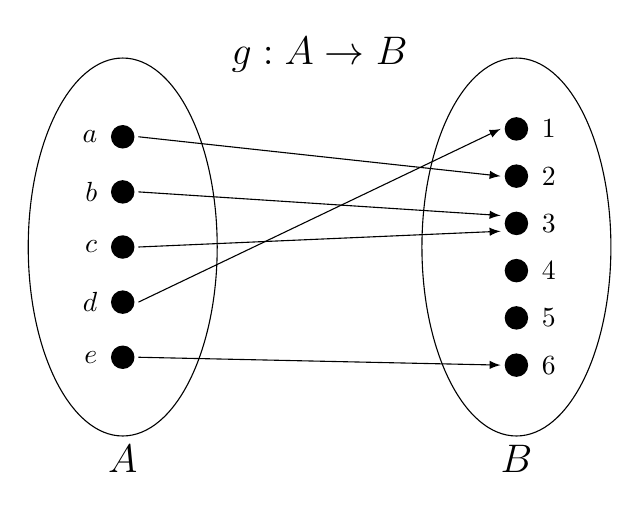
\begin{tikzpicture}[scale=1]
        \foreach \x in  {1,...,6}
        {
            \node at (5, -\x*0.6)[circle,fill,inner sep=3pt]{};
            \draw[shift={(5.2, -\x*0.6)}] node[right] {$\x$};
        }
        \draw (5,-2.1) ellipse (1.2 and 2.4);

        \foreach \x/\s in  {1/a,2/b,3/c,4/d,5/e}
        {
            \node at (0, -\x*0.7)[circle,fill,inner sep=3pt]{};
            \draw[shift={(-0.2, -\x*0.7)}] node[left] {$\s$};
        }
        \draw (0,-2.1) ellipse (1.2 and 2.4);

        \draw[-latex] (0.2,-0.7) -- (4.8,-1.2); 
        \draw[-latex] (0.2,-1.4) -- (4.8,-1.7); 
        \draw[-latex] (0.2,-2.1) -- (4.8,-1.9); 
        \draw[-latex] (0.2,-2.8) -- (4.8,-0.6); 
        \draw[-latex] (0.2,-3.5) -- (4.8,-3.6);
        
        \node[below] at (0, -4.5){\Large $A$};
        \node[below] at (5, -4.5){\Large $B$};
        \node[above] at (2.5, 0){\Large $g:A \to B$};
    \end{tikzpicture}}
\end{center}

然而,这在某种程度上确实\emph{代表}了函数的概念。在这幅图中,我们用椭圆分别表示了定义域 $A$ 和值域 $B$。$A$ 和 $B$ 的元素则用椭圆内的点来表示,并且进行了标记。我们根据函数 $g: A \to B$ 在这些点之间画上箭头。

这种方法通常用于探索函数的特性,或者构造反例来反驳某个主张。通过绘制一些点和箭头,并尝试它们的连接方式,我们可以逐步构建一个例子的基础\emph{结构}。然后,再为图中的各部分分配名称和公式,使其更加严谨。

在我们的讨论中,我们会用一些示意图来说明某些属性和概念,同时提供更严谨的陈述或描述。我们鼓励你也采用这种方法。